\chapter{Resultados}
\label{ch:Resultados}
\section{Resultados parciais}
\section{Abstrair o problema no contexto}
O contexto geral do trabalho é projetar e construir um sistema AM para auxiliar no diagnóstico da doença de Parkinson, utilizando sinais obtidos por dispositivos sEMG, e o problema principal gira em torno de como esse sistema será desenvolvido. Por se tratar da construção de um software, isso necessita de um planejamento prévio de como será feita essa construção, levando em consideração um conjunto de variáveis para tomada de decisões. Neste trabalho o sistema a ser desenvolvido se trata de um sistema AM, que requer uma maior atenção sobre algumas variáveis, como quantidade de recursos e tipos de dados obtidos, sendo que essas variáveis servem como indicadores para auxiliar a decisão de qual algoritmo utilizar para se encontrar a melhor solução possível para esse problema.

\section{Prova de conceito}
Para verificar a viabilidade do projeto, além de buscar entender o funcionamento da biblioteca \textit{scikit-learn}. Realizou-se uma prova de conceito, desenvolvendo um algoritmo utilizando o SVM, para predizer os dados relacionados a uma porta lógica XOR. Foram utilizados também o \textit{numpy} para as manipulações matemáticas e o \textit{matplotlib} para plotar o gráfico. Para o teste utilizou-se 500 amostras. Sendo que estas foram separadas em 75\% em dados de treino e os 25\% restantes em dados de teste. Ou seja, 125 dados de treino e 375 dados de teste, não utilizou-se dados de validação.

Como observado na Figura \ref{svmxor} na página \pageref{svmxor}, o svm conseguiu separar corretamente a maioria dos dados, sendo que, na imagem as bolas laranjas equivalem ao valor esperado “1”, e as bolas azuis equivalem ao valor esperado “0”. Já os contornos equivalem ao valor atingido pelo SVM, ou seja, as bolas dentro da área roxa foram preditas como “0” e  a bolas na área laranjada foram preditas como “1”. Também é possível observar nessa imagem os hiperplanos de separação.

Utilizou-se também para verificar a precisão do modelo, a matriz de confusão, como pode ser observado na Figura \ref{mcxor} na página \pageref{mcxor}, e na Figura \ref{mcxornormalizada} na página \pageref{mcxornormalizada}, a qual mostra a matriz de confusão normalizada com a porcentagem de dados.

Outra ferramenta utilizada foi a \textit{Classification report} Figura \ref{class_report} na página \pageref{class_report}, que descreve separadamente a taxa de precisão, além de outros conceitos da estatística.

\begin{figure}[!htb]
	\centering
	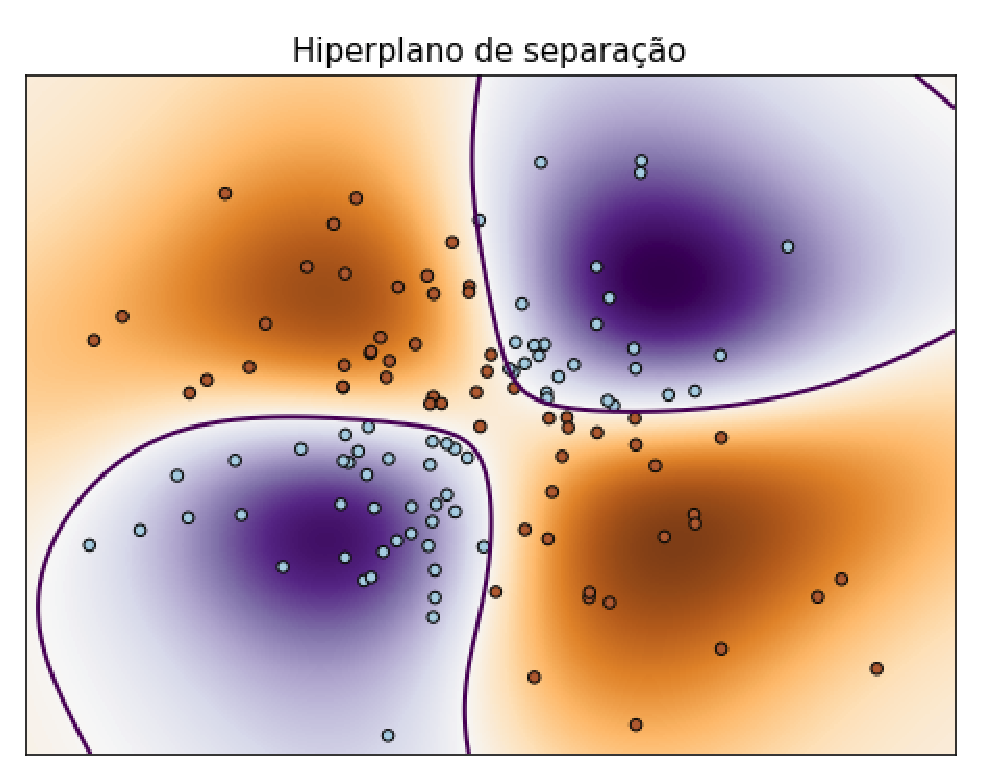
\includegraphics[width=0.8\textwidth]{figuras/xor.eps}
	\caption{Hiperplano de separação do SVM na porta XOR.}
	\label{svmxor}
\end{figure}

\begin{figure}[!htb]
	\centering
	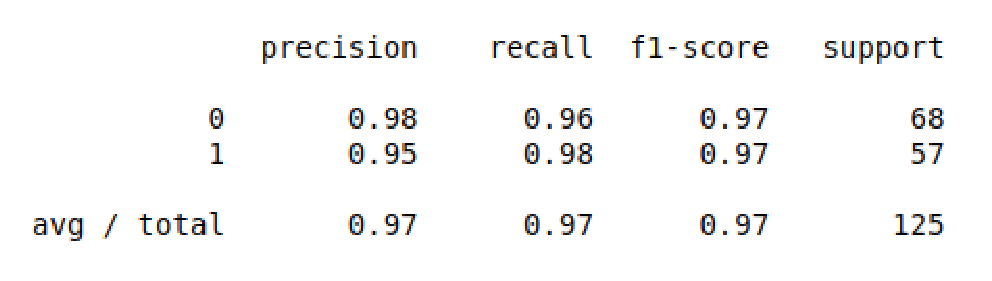
\includegraphics[width=0.8\textwidth]{figuras/class_report.eps}
	\caption{\textit{Classification report} da porta XOR.}
	\label{class_report}
\end{figure}

\begin{figure}[!htb]
	\centering
	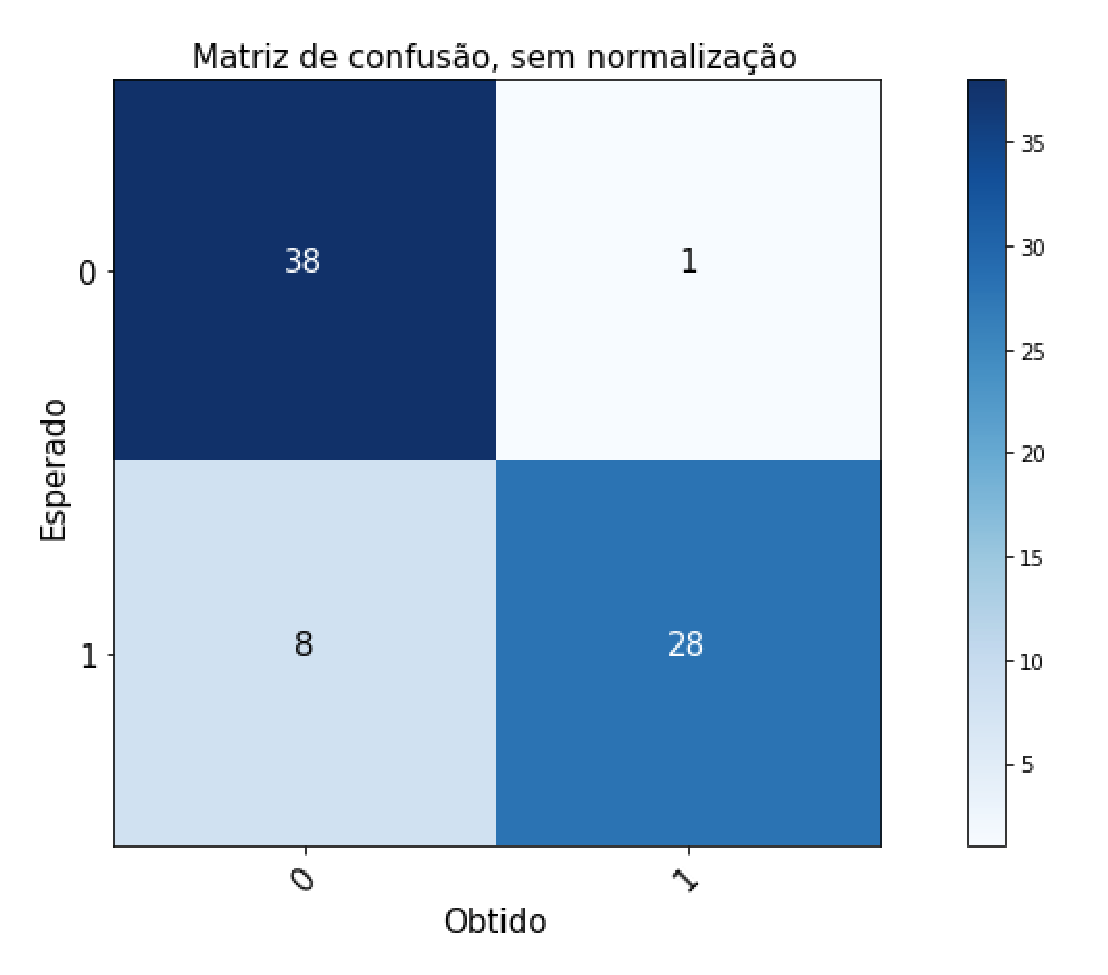
\includegraphics[width=0.8\textwidth]{figuras/mcxor.eps}
	\caption{Matriz de confusão da porta XOR.}
	\label{mcxor}
\end{figure}

\begin{figure}[!htb]
	\centering
	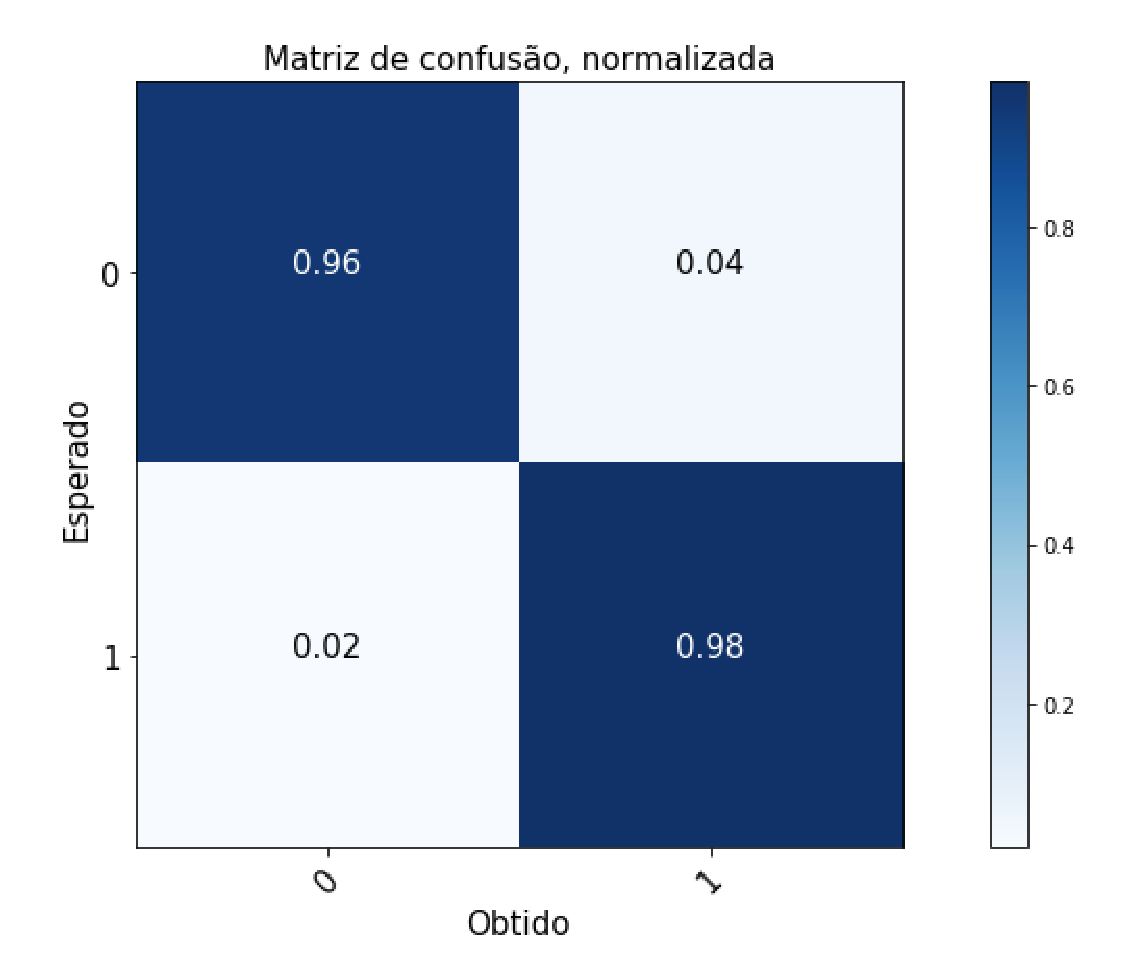
\includegraphics[width=0.8\textwidth]{figuras/mcxornormalizada.eps}
	\caption{Matriz de confusão normalizada da porta XOR.}
	\label{mcxornormalizada}
\end{figure}
